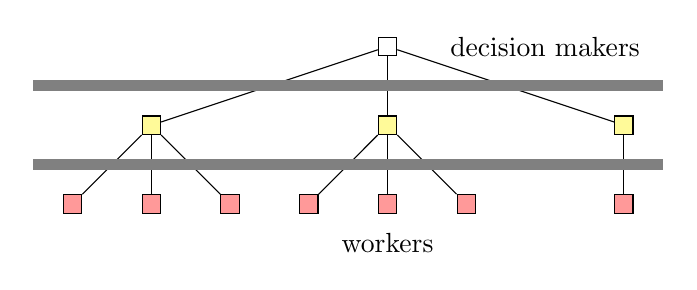
\begin{tikzpicture}[
>=stealth,
line/.style={draw},
bigl/.style={draw,line width = 4pt, color=black!50},
root/.style={draw},
func1/.style={draw,fill=yellow!40},
func2/.style={draw,fill=red!40},
]

\node[root] (root) at (0,0) {};

\node[func1] (fu1) at (-3,-1) {};
	\node[func2] (fu12) [below of = fu1] {};
	\node[func2] (fu13) [right of = fu12] {};
	\node[func2] (fu14) [left of = fu12] {};

\node[func1] (fu2) at (0,-1) {};
	\node[func2] (fu22) [below of = fu2] {};
	\node[func2] (fu23) [right of = fu22] {};
	\node[func2] (fu24) [left of = fu22] {};

\node[func1] (fu3) at (3,-1) {};
	\node[func2] (fu31) [below of = fu3] {};

\path[line] (root) -- (fu1);
	\path[line] (fu1) -- (fu13);
	\path[line] (fu1) -- (fu12);
	\path[line] (fu1) -- (fu14);

\path[line] (root) -- (fu2);
	\path[line] (fu2) -- (fu22);
	\path[line] (fu2) -- (fu23);
	\path[line] (fu2) -- (fu24);

\path[line] (root) -- (fu3);
	\path[line] (fu3) -- (fu31);

%separators
\path[bigl] (-4.5,-.5) -- (3.5,-.5);
\path[bigl] (-4.5,-1.5) -- (3.5,-1.5);

%functions
\node (fun1) at (2,0) {decision makers};
\node (fun2) at (0,-2.5) {workers};



\end{tikzpicture}